\section{Q-GPU}
\label{sec:qgpu}

\begin{figure}[t!]
    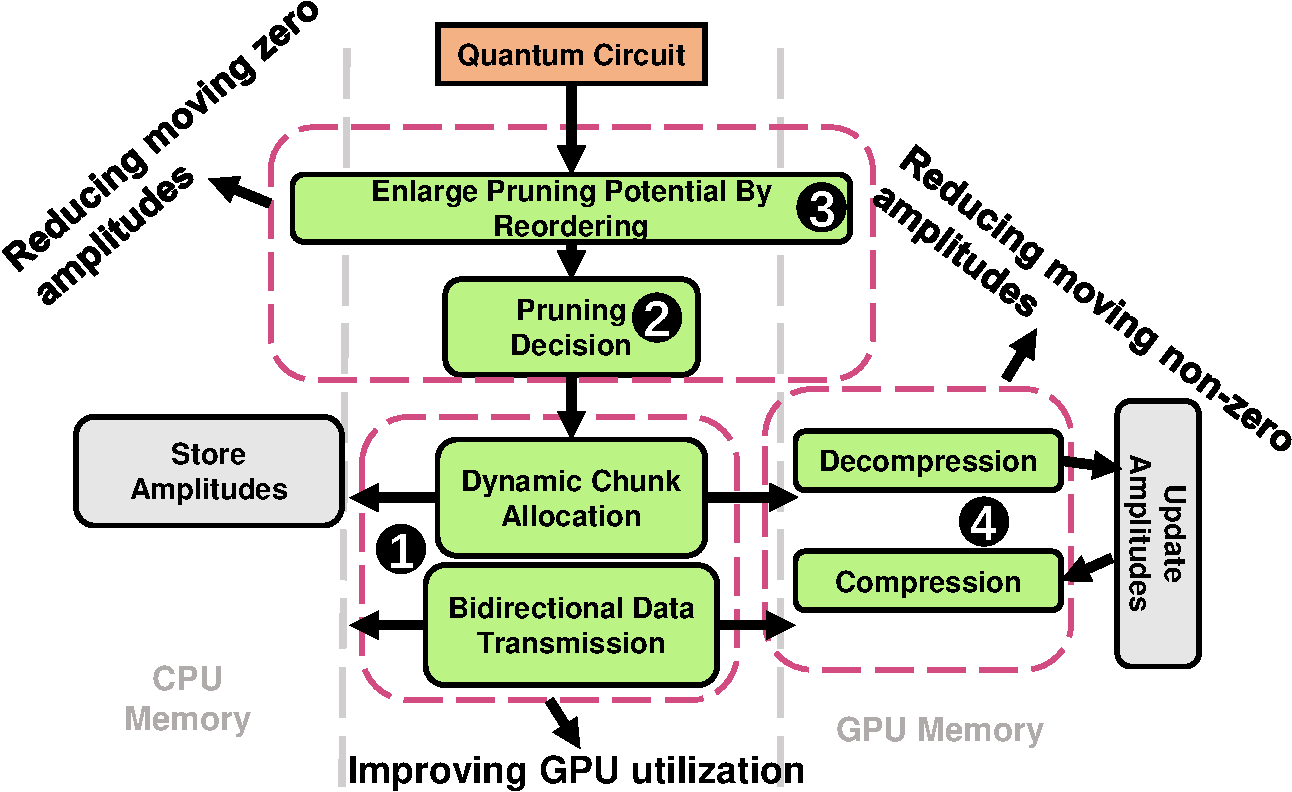
\includegraphics[width=\textwidth]{Images/appendix2/section-4/overview.pdf}
    \centering
    \caption{High level overview of Q-GPU.}
    \label{fig-5}
    \vspace{-5pt}
\end{figure}

In this paper, we propose {\it Q-GPU}, a framework that features several end-to-end optimizations. Figure~\ref{fig-5} depicts the high-level overview of Q-GPU. (\circled{1}) Q-GPU performs proactive state amplitude transfer to fully utilize the bi-directional data transfer bandwidth between CPU and GPU (Section \ref{sec:overlap}). (\circled{2}) Before copying state amplitudes to GPU, Q-GPU performs dynamic redundancy elimination that prunes zero state amplitudes to avoid unnecessary data movements (Section \ref{sec:pruning}). (\circled{3}) Q-GPU features a compiler-assisted, dependency-aware quantum gate reordering to enlarge the potential of pruning (i.e., the number of zero amplitudes). (\circled{4}) Q-GPU implements a GPU-supported, lossless amplitude compression to further reduce the data transfer caused by non-zero state amplitudes with minimal runtime overheads (Section \ref{sec:compress}).

\subsection{Proactive State Amplitudes Transfer}
\label{sec:overlap}

In the naive execution, one reason behind the poor GPU utilization is the sequential state amplitude transfer between CPU and GPU. Specifically, when the GPU finishes updating all local chunks, those chunks are first copied back to CPU memory before the CPU can transfer the next batch of un-updated chunks to the GPU. This restriction is reasonable in the scenarios when particular chunks are involved in consecutive updates since the chunks being copied from the GPU's memory cannot be overwritten during the copying. In other words, data movements are synchronized to avoid data conflicts.
However, if the subsequent chunks from the CPU are not copied to the same memory locations on the GPU where current chunks are stored, such data conflict does not exist. As a result, one can transfer the chunks simultaneously from the CPU to the GPU and from the GPU to the CPU.

In our work, Q-GPU leverages CUDA streams to enable concurrent and bi-directional chunk copy to fully utilize the available bandwidth between the CPU and GPU. To avoid potential data conflict, Q-GPU implements two CUDA streams and partitions the GPU memory into two halves. One stream is responsible for the first half partition that acts as a buffer holding the chunks the GPU is currently updating. The other stream is responsible for the second half partition that acts as a buffer for ``prefetching'' the next chunks for the GPU to update. The two memory partitions work as ``circular buffers'' to feed the GPU with the required chunks. These two streams can potentially overlap and execute concurrently. 

\par Figure \ref{fig:timeline-overlap} illustrates the timeline of the baseline and each of our optimizations. The proposed proactive state amplitude transfer (\circledwhite{III}) achieves \circled{A} cycles savings compared with the baseline (\circledwhite{I}). We also show that the naive approach (\circledwhite{II}) performs worse than the baseline. 

\begin{figure}[t!]
    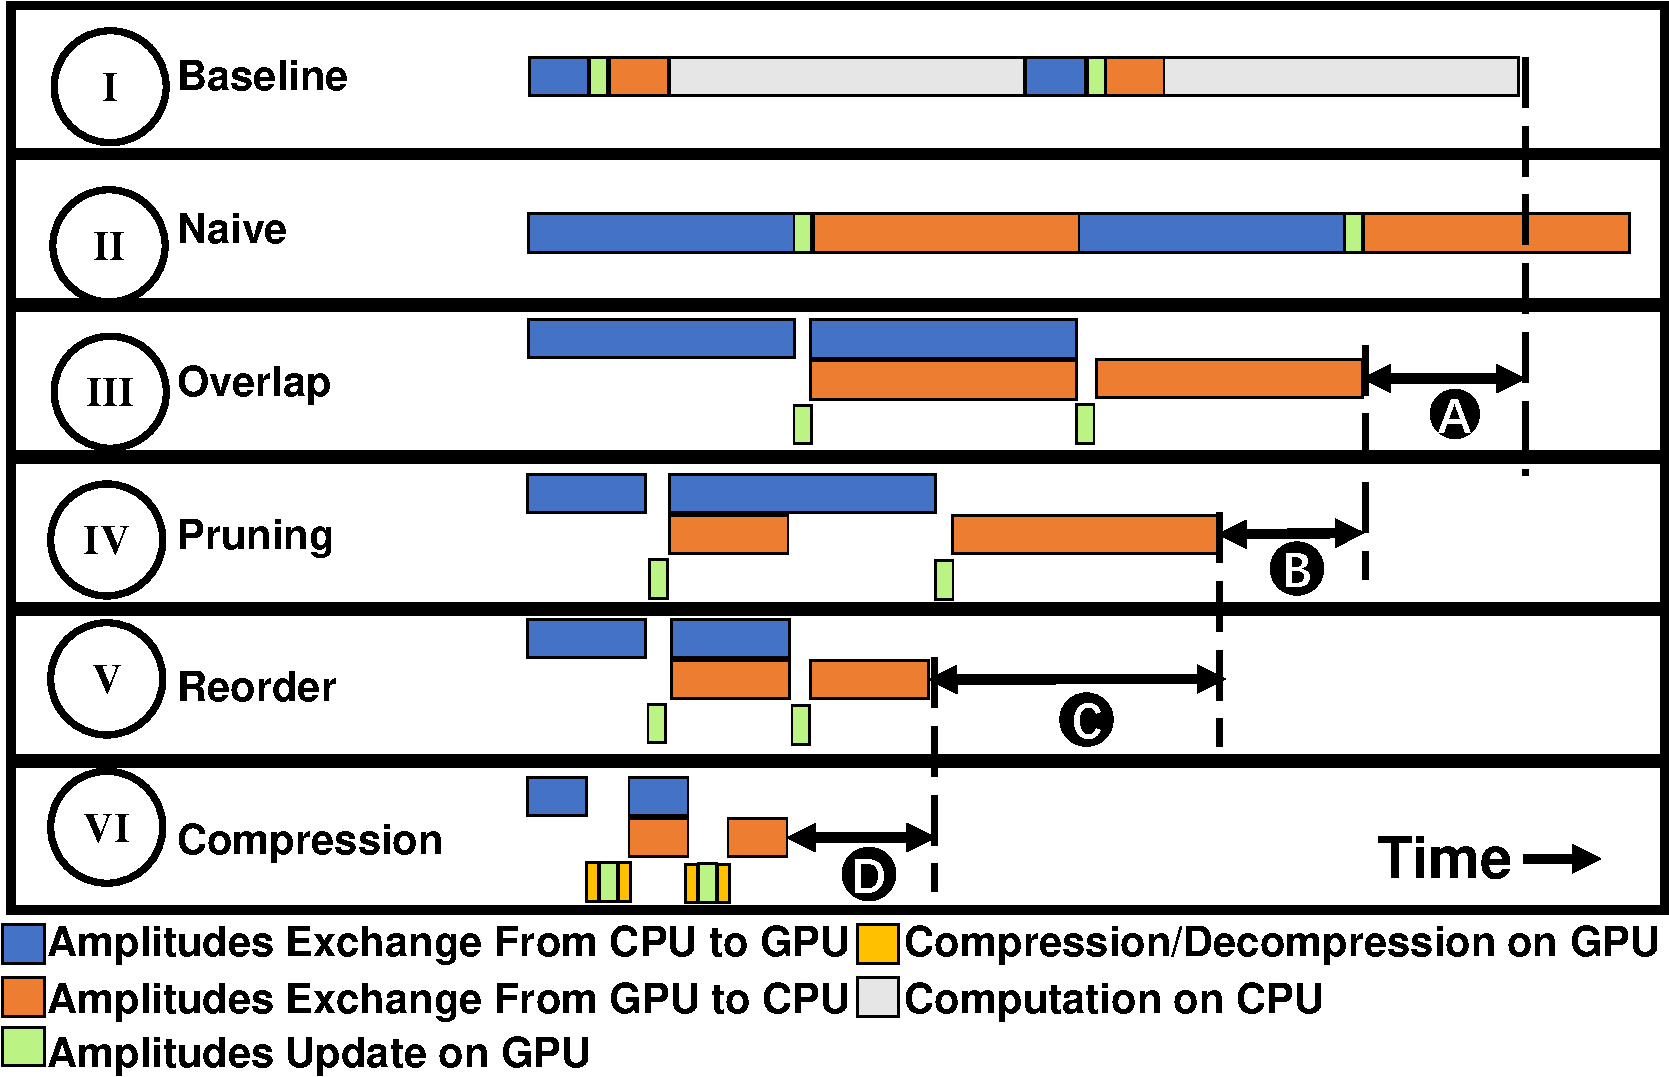
\includegraphics[width=\textwidth]{Images/appendix2/section-4/timeline.pdf}
    \centering
    \caption{Time-line graph showing the benefits of each optimization in Q-GPU.}
    \label{fig:timeline-overlap}
    \vspace{-5pt}
\end{figure}

\subsection{Pruning Zero State Amplitudes}
\label{sec:pruning}
\noindent While overlapping improves the bandwidth utilization, the total amount of amplitudes that are transferred remains unchanged. 
To reduce the data movement, we observe that there exist a considerable amount of zero state amplitudes that do not need to be updated during simulation.
Thus, those zero state amplitudes can be pruned before transferring the chunks. 
 
\noindent \textbf{Source of zero amplitudes:}
Let us assume there are $n$ qubits, the initial states are usually set as $|0\rangle^{\otimes{n}}$ in the general QCS, indicating that all qubits have zero probability of being measured as $|1\rangle$. 
Hence, all state amplitudes are zeros, except for $a_{0_{1}0_{2}\dots0_{n}}$ which is 1. As the state of a particular qubit is unchanged until an operation is being applied on it, its state remains $|0\rangle$ until that operation happens. 
For instance, if a particular qubit $q_k$ is $|0\rangle$, all the state amplitudes $a_{\times\dots\times1_{k}\times\dots\times}$ are zeros since $q_k$ has zero probability to be measured as $|1\rangle$. 
In general, if $m$ of $n$-qubits are not involved, amplitudes $a_{\times{0_{k_1}}\times{0_{k_2}}\dots\times{0_{k_m}}\times\times}$ are possible to be non-zero values, whereas the remaining amplitudes are guaranteed to be zero values, i.e. $2^n-2^{n-m}$ amplitudes are zero values.
Therefore, even if only one qubit is not involved, then half of the state amplitudes are zeros. 

\noindent \textbf{Pruning potential:}
To investigate the potential of pruning, Table \ref{tab-inv} lists the number of total operations and the number of operations before all qubits are involved. For circuits like {\tt iqp}, we can expect a significant reduction of data movement after pruning since many qubits are not involved until the end of execution. However, for {\tt qft} and {\tt qf}, all qubits are involved at the beginning of execution, diminishing the potential of pruning benefits.  
We also use {\tt hchain\_18} as an example and plot the distribution of state amplitudes after each operation (i.e., quantum gate) being applied in a quantum circuit. 
Figure \ref{fig:hchain18state} shows the state amplitude distribution after 0, 30, 60 and 90 operations. One can observe that a large portion of state amplitudes are zeros at the beginning of the simulation. During simulation, the amplitudes are gradually updated to non-zero values since more qubits are involved. 

\begin{figure*}[h!]
    \centering
    \subcaptionbox{\label{fig:step0}}[.22\textwidth]{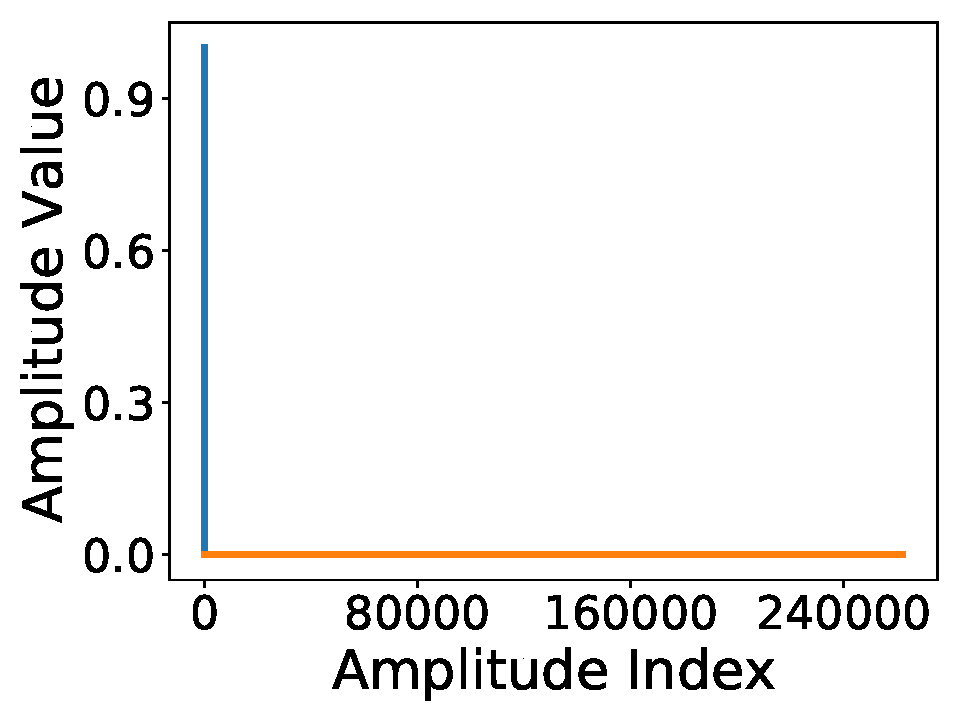
\includegraphics[width=0.22\textwidth]{Images/appendix2/section-4/state_vec_0.pdf}}
    \hspace{-5pt}
    \subcaptionbox{\label{fig:step30}}[.22\textwidth]{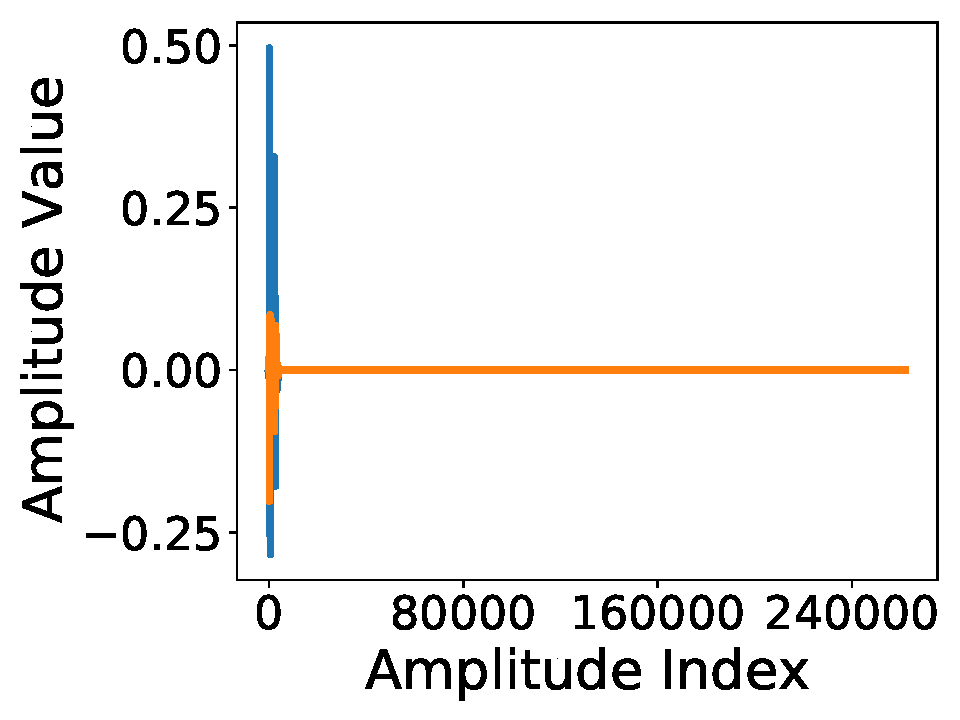
\includegraphics[width=0.22\textwidth]{Images/appendix2/section-4/state_vec_30.pdf}}
    \subcaptionbox{\label{fig:step60}}[.22\textwidth]{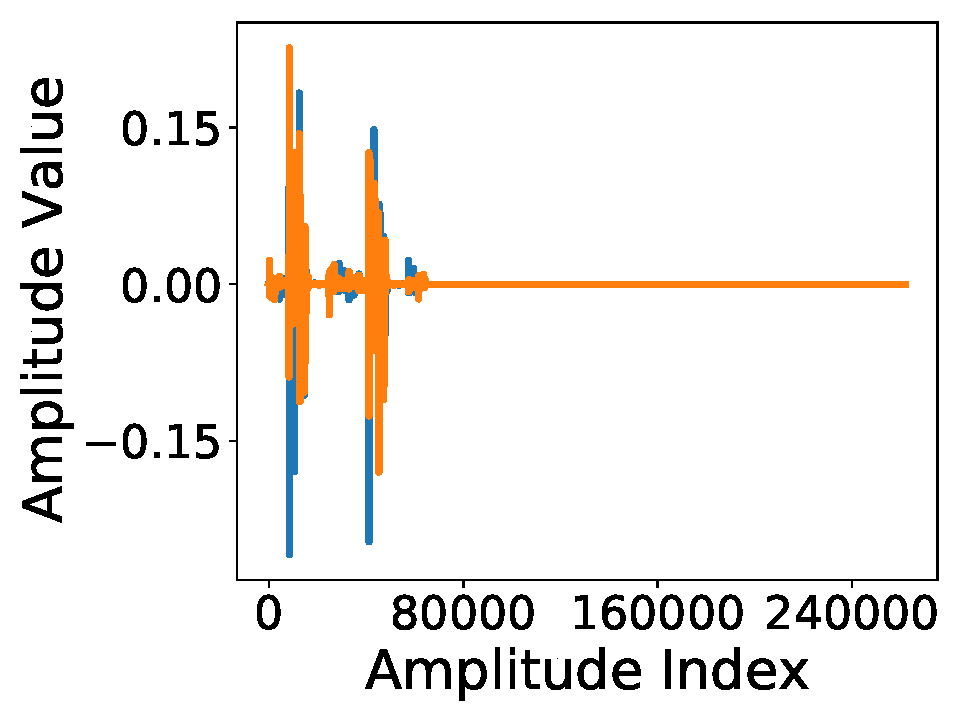
\includegraphics[width=0.22\textwidth]{Images/appendix2/section-4/state_vec_60.pdf}}
    \vspace{-5pt}
    \subcaptionbox{\label{fig:step90}}[.22\textwidth]{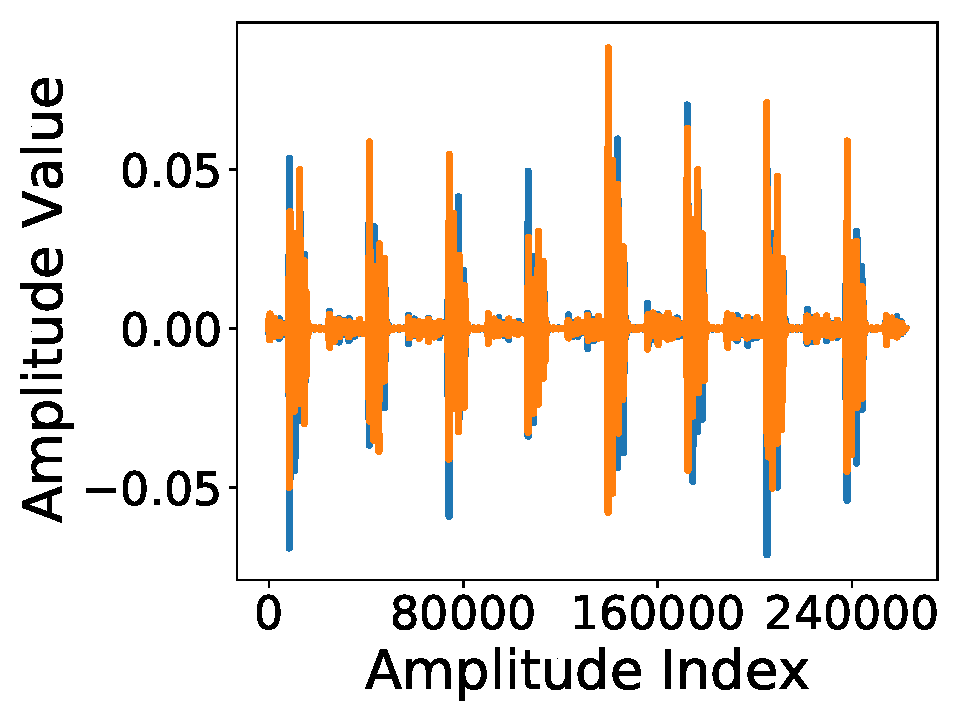
\includegraphics[width=0.22\textwidth]{Images/appendix2/section-4/state_vec_90.pdf}}
    \vspace{-5pt}
    \caption{State amplitudes distribution of {$\tt hchain\_18$}, after 0, 30, 60 and 90 operations from left to right. Blue and orange lines denote real and imaginary parts of an amplitude respectively.}
    \vspace{-5pt}
\label{fig:hchain18state}
\end{figure*}

\par In general, let us assume we have an operation involving $m$ states, if all of the states are zero, these $m$ states remain zeros after applying any operation. As a result, we do not need to transfer the zero state amplitudes to the GPU as their values will not change. Therefore, one can reduce the data movement between CPU and GPU by  pruning the zero state amplitudes. One intuitive approach is to check each state value by traversing all states. However, a more efficient approach can be adopted, as we illustrate below.


\begin{table}[t!]
\centering
%\scriptsize
\caption{The number of total operations and the number of operations before all qubits are involved for all circuits with 34 qubits.}
\begin{tabular}{||c|c|c||} 
 \hline
 Circuit & Total Operations & Operations Before Completely Involved  \\ [0.5ex] 
 \hline\hline
 {\tt hchain} & 1786 & 272 \\ 
 \hline
 {\tt rqc} & 124 & 54 \\
 \hline
 {\tt qaoa} & 754 & 19 \\
 \hline
 {\tt gs} & 37 & 16 \\
 \hline
 {\tt hlf} & 48 & 16 \\
 \hline
 {\tt qft} & 184 & 13 \\
 \hline
 {\tt iqp} & 146 & 132 \\
 \hline
 {\tt qf} & 222 & 16 \\ [1ex] 
 \hline
\end{tabular}
\label{tab-inv}
\end{table}

\noindent \textbf{Pruning Mechanism: }In the proposed Q-GPU, we use bits in a binary string as flags to indicate whether a qubit has been involved after a set of gate operations (denoted as $involvement$ in Algorithm \ref{alg:pruning}). Initially, all the bits in $involvement$ are set to 0. When $q_k$ is involved, the $k$th bit in $involvement$ is set to 1. Recall that the state vector is partitioned into chunks, the index of a chunk, i.e., $iChunk$, determines whether a chunk will be transferred or not. 
To compare $iChunk$ with flag bits in $involvement$, we define $iChunk^{\prime}$ as the left-shifted $iChunk$ to align with $involvements$. When $iChunk^{\prime}$ is larger than $involvement$, it indicates that at least one bit of $iChunk^{\prime}$ is 1 and the corresponding flag bit in $involvement$ is 0. In this situation, the corresponding qubit (i.e., indexed by this flag bit) has not been involved by any operation. 
As such, we skip the remaining chunks and stop the iteration (line 5). On the other hand, if $iChunk^{\prime}$ is smaller than or equal to $involvement$, the redundancy within a chunk is determined by $iChunk^{\prime}$ \& $involvement$ (line 8). 
For a qubit whose corresponding bit in $iChunk^{\prime}$ is 1, if it has already been involved by previous operations, its corresponding bit in $involvement$ is also 1. 
Therefore, for all the qubits that is 1 in $iChunk^{\prime}$, if all of them have already been involved by previous operations, $iChunk^{\prime}$ $\&$ $involvement$ results in $iChunk^{\prime}$ itself. Otherwise, all the state amplitudes within this chunk are zeros, and we can prune this chunk. Moreover, the $chunkSize$ here is dynamically determined rather than a statically fixed value, which enhances the benefit of the above-discussed strategy. Specifically, we select $chunkSize$ by finding the least non-zero bit of $involvement$. 
This is useful, especially at the beginning of the simulation where many state amplitudes are zeros. For instance, assuming we have an 8-qubit circuit and the $involvement$ flag is $00000011$ at the early execution stage, the $chunkSize$ is dynamically set to 2, which has fewer zeros within a chunk compared to a larger chunk. The $involvement$ flag bits are updated according to the qubits involved in each operation (line 14). In Figure \ref{fig:timeline-overlap}, the proposed pruning mechanism (\circledwhite{IV}) further saves (\circled{B}) cycle over \circledwhite{III}.  


\begin{algorithm}[t!]
%\scriptsize
\SetKwFunction{memCpy}{memCpy}
\SetKwFunction{Exe}{execute}
\SetKwFunction{Update}{updateInvolvement}
\SetKwFunction{Get}{getChunkSize}
    \SetKwInOut{KwIn}{Variable list}
    \SetKwInOut{KwOut}{Output}
    \KwIn{\makebox[1.5cm]{$N$} Total chunks number in CPU, \\
    \makebox[1.5cm]{$involvement$} Flag indicating which qubits are involved}
	
	\tcc{Determine $chunkSize$ by locating the least non-zero bit of $involvement$}
	$chunkSize$, $N$ = \Get{involvement}\\
   	\For	{$iChunk\gets0$ \KwTo $N-1$} {
   		$iChunk^{\prime} = iChunk << chunkSize$\\
   		\If {$iChunk^{\prime} > involvement$  } {
   			break
   		}
   		\If {$iChunk^{\prime} \& involvement \neq iChunk^{\prime}$} {
   			continue
   		}
   		\tcc{Amplitudes update}
   		\dots\\
   	}
	\Update{involvement}
    \caption{Pruning zero state amplitudes.}
    \label{alg:pruning}
\end{algorithm}

\subsection{Reordering to Delay Qubit Involvement}
\label{sec:reorder}

\begin{figure}[h!]
    \centering
    \subcaptionbox{\label{fig:orgorder}}[.3\textwidth]{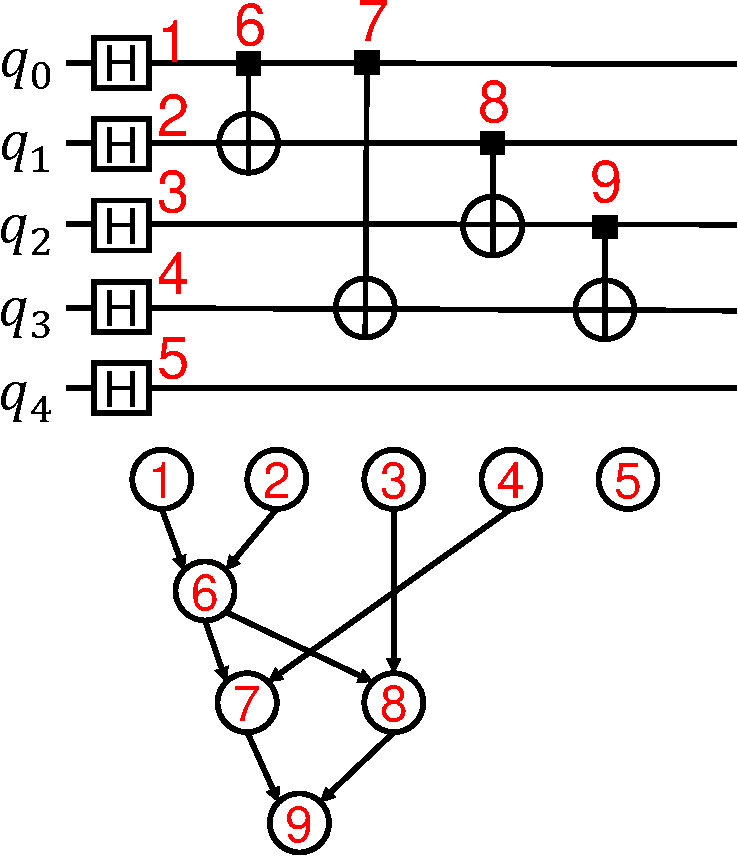
\includegraphics[width=0.3\textwidth]{Images/appendix2/section-4/orgorder.pdf}}
    \hspace{0pt}
    \subcaptionbox{\label{fig:greedyorder}}[.3\textwidth]{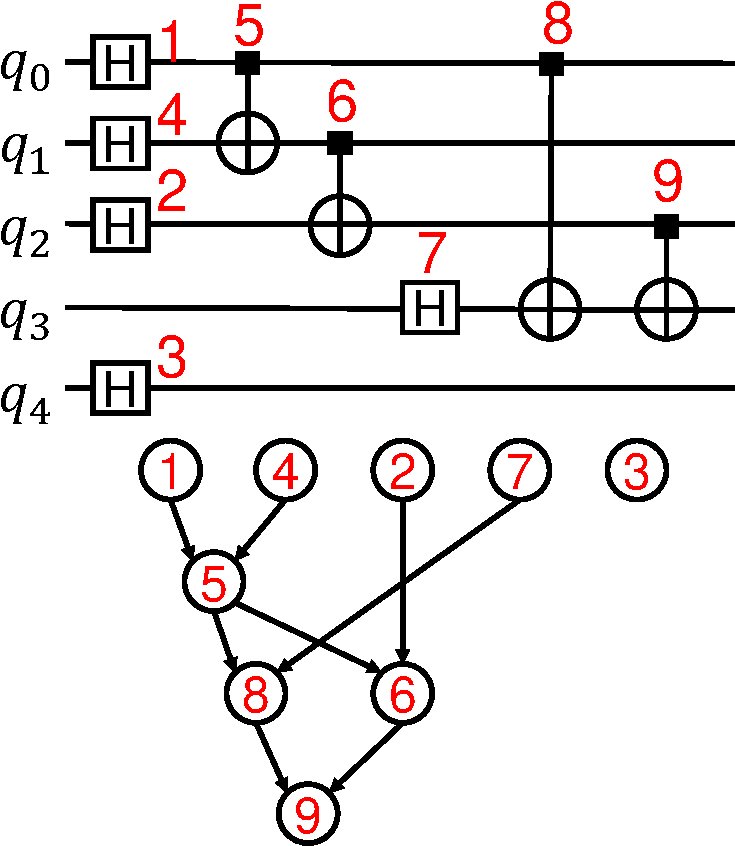
\includegraphics[width=0.3\textwidth]{Images/appendix2/section-4/greedyorder.pdf}}
    \subcaptionbox{\label{fig:forwardorder}}[.3\textwidth]{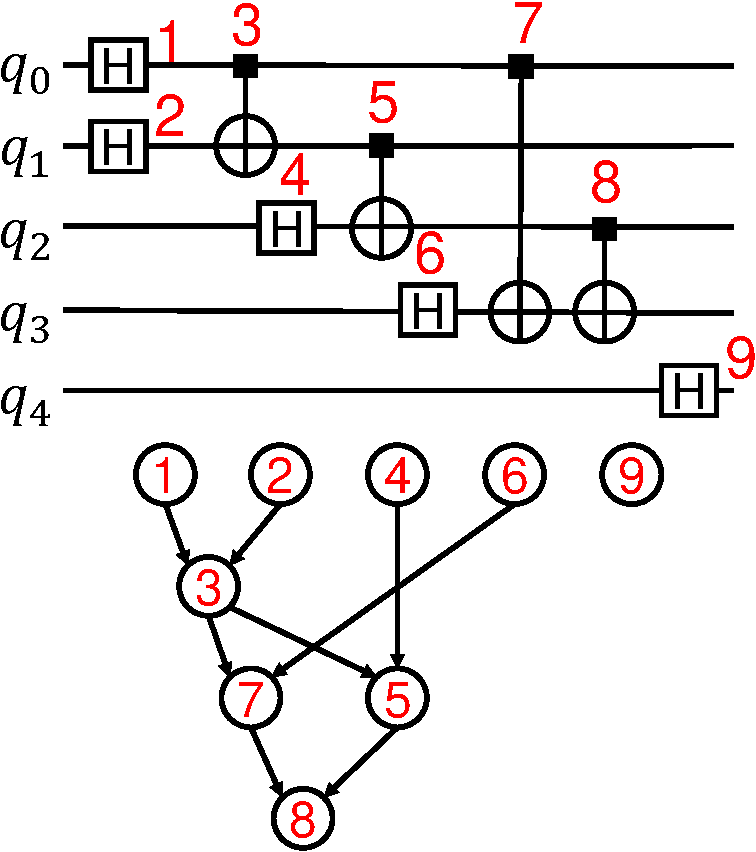
\includegraphics[width=0.3\textwidth]{Images/appendix2/section-4/forwardorder.pdf}}
    \vspace{00pt}
    \caption{A walk-through example to illustrate the reordering benefits using ${\tt gs\_5}$. The red number denotes the operation orders before and after reordering.}
    \vspace{0pt}
\label{fig:reorder}
\vspace{-5pt}
\end{figure}

\noindent  
In order to enlarge the potential of pruning, such that more state amplitudes are zeros during simulation, we propose compiler-assisted, dependency-aware quantum operation reordering to delay the involvement of qubits. 
Specifically, when applying a gate, we choose the one that incurs the minimum number of additional qubits to be involved with those qubits that have been already involved by previous operations. 
For example, Figure~\ref{fig:orgorder} shows the {\tt gs\_5} circuit in the original execution order. The first five gates are $H$ gates, where each gate applies to an individual qubit. As a result, once these gates have been applied, all the five qubits are involved.
The next operation is a CNOT gate applied to qubits $q_{0}$ and $q_{1}$ ($CNOT_{6}$). All the state amplitudes are likely non-zero because the qubits are involved by the $H$ gates. Therefore, applying this CNOT gate requires updating all the non-zero amplitudes in the state vector, leading to moving and traversing the entire state vector on the GPU. However, the $CNOT_{6}$ can be executed before some of the $H$ gates without violating the circuit semantics. This gate reordering allows more zero state amplitudes (fewer data movements) when simulating the $CNOT_{6}$ gate. 
It is also important to emphasize that any reordering must ensure that the gate dependencies are presented. For instance, $CNOT_{6}$ and $CNOT_{7}$ cannot be reordered due to the dependency on $q_0$.

To this end, we propose a compiler-assisted optimization to reorder the gate sequence with the goal of delaying the qubit involvement. Specifically, gates that are applied on different qubits in a quantum circuit can be executed independently in any order and the execution sequence of these independent gates does not affect the final simulation result~\cite{10.1145/3297858.3304023,10.1109/HPCA51647.2021.00026,10.1145/3498325}. This provides us the opportunity to reorder the independent gates, we use a directed acyclic graph (DAG) to represent the gate dependency in a circuit. Based on the DAG, we reorder the independent gates such that the simulation sequence involves the minimum number of new qubits when simulating each gate. Specifically, we investigate two heuristic strategies: 1) greedy reordering, and 2) forward-looking reordering.

\begin{algorithm}[t!]
%\scriptsize
\SetKwFunction{getCost}{getCost}
\SetKwFunction{append}{append}
\SetKwFunction{erase}{erase}
\SetKwFunction{numPre}{numPredecessors}
\SetKwFunction{desc}{descendants}
    \SetKwInOut{KwIn}{Input}
    \SetKwInOut{KwOut}{Output}

    \KwIn{\makebox[1.5cm]{$DAG$} A DAG representing circuit dependencies.}
    \KwOut{
    \makebox[1.5cm]{$gatesList$} List of gates after reordering,\\
    }

    $gatesList = [\ ]$\\
    $exeList = [\ ]$\\
    \tcc{First we build $DAG$ and push gates without predecessors to an execution list}
    \For {$g$ in $DAG$}{
    	\If {$g.\numPre{} == 0$}{
    		$exeList.\append{g}$
    	}
    }
	
	\tcc{Then we traverse DAG in topological order and greedily decides the execution order of the gates}
	\While {$exeList \neq \emptyset$ } {
		$nextGate = NULL$ \\
		$minCost = 0$ \\
		\For {$g$ in $exeList$} {
			$cost = g.\getCost{}$ \\
			\If {$cost < minCost$} {
				$minCost = cost$\\
				$nextGate = g$\\
			}
		}
		$exeList.\erase{nextGate}$ \\
		$gatesList.\append{nextGate}$ \\
		\For {$g$ in $nextGate.\desc{}$} {
			$g.\numPre{} = g.\numPre{} - 1$ \\
			\If {$g.\numPre{} == 0$} {
				$exeList.\append{g}$
			}
		}
	}
	
    \caption{Quantum operation reorder.}
    \label{alg-3}
\end{algorithm}

\noindent\textbf{Greedy reordering:} greedy reordering traverses the DAG in topological order and greedily selects the gate (i.e., node in the DAG) that introduces the minimum number of new qubits to the list of updated qubits.
The details of this method are illustrated in~Algorithm~\ref{alg-3}. First, gates without predecessors in the DAG can be executed at the first steps and are put into $exeList$. Second, we traverse the gates in $exeList$ and find the one that introduces the minimum number of newly involved qubits (lines 13 to 19). Then, we remove this gate from $exeList$ and append it to the list of re-ordered gates. Third, we traverse the descendants of this gate and if a descendant does not have any predecessors other than this current gate, it will be added to $exeList$ (lines 22 to 27). The second and the third steps are repeated until $exeList$ is empty.
In the rest of this section, we use Figure \ref{fig:orgorder} as the example to illustrate how we perform reordering. 
At first, the $exeList$ is [$g_1$, $g_2$, $g_3$, $g_4$, $g_5$]. Since each of these five gates involves one new qubit, we randomly select one gate among them to start simulation. In this example, $g_1$ is selected as the starting gate. After traversing all its descendants, no new gates can be added into $exeList$. 
Next, the $exeList$ becomes [$g_2$, $g_3$, $g_4$, $g_5$].
In the next three steps, we randomly select $g_3$, $g_5$ and $g_2$ since no new gates can be executed and all gates in $exeList$ have equal priority. Then the $exeList$ becomes [$g_4$, $g_6$]. 
At this time, $involvedQubits$ is [$q_0$, $q_1$, $q_2$, $q_4$]. Therefore, $g_4$ involves one new qubit ($q_3$), whereas $g_6$ will not introduce any new qubits since it acts on $q_0$ and $q_1$ that are already in the involved list. 
Therefore, we will greedily select $g_4$ to execute since it involves the least new qubits. 
One can follow these reordering steps to reach the new ordering shown in Figure~\ref{fig:greedyorder}.
As a result, the number of involved qubits at each step is 1 $\to$ 2 $\to$ 3 $\to$ 4 $\to$ 4 $\to$ 4 $\to$ 5 $\to$ 5 $\to$ 5. Since the baseline is 1 $\to$ 2 $\to$ 3 $\to$ 4 $\to$ 5 $\to$ 5 $\to$ 5 $\to$ 5 $\to$ 5, the final involvement is delayed by two steps.
However, a better solution for reordering is to select $g_2$ and $g_6$ in the second and the third step, since applying these two gates only adds one qubit to $exeList$, while applying $g_3$ and $g_5$ adds two. Thus greedy reordering may misses the optimal choice.

\begin{algorithm}[t!]
%\scriptsize
\SetKwFunction{getCost}{getCost}
\SetKwFunction{qubits}{qubits}
\SetKwFunction{Push}{push}
\SetKwFunction{insert}{insert}
\SetKwFunction{erase}{erase}
\SetKwFunction{desc}{descendants}
\SetKwFunction{numPre}{numPredecessors}
    \SetKwInOut{KwIn}{Input}
    \SetKwInOut{KwOut}{Output}

    \KwIn{
	\makebox[1.5cm]{$g$} Gates from $exeList$, \\
    \makebox[1.5cm]{$exeList$} List of gates that are executable, \\
    \makebox[1.5cm]{$involvedQubits$} Set of qubits which have already been acted on.
	}
    \KwOut{\makebox[1.5cm]{$cost$} Potential involved qubits after executing $g$.}
	
	$costCurrent = 0, costLookAhead = 0$\\
	
    \tcc{First we compute additional qubits that will be acted on by executing current gate}
    \For {$q$ in $g$.\qubits{}} {
    	\If {$q$ not in $involvedQubits$} {
    		$costCurrent = costCurrent + 1$\\
    		$involvedQubits.\insert{q}$		 
    	}
    }
    
    $exeList.\erase{g}$\\
    \For {$g^\prime$ in $g.\desc{}$} {
    	\If {$g^\prime$.\numPre{} == 1} {
    		$exeList$.\Push{$g^\prime$}
    	}
    }
	
	\tcc{Then we traverse current $exeList$ and compute the cost of selecting a gate that involve least additional qubits}
	\For {$g^{\prime\prime}$ in $exeList$} {
		$curCostLookAhead = 0$ \\
		\For {$q^\prime$ in $g^{\prime\prime}$.\qubits{}} {
			\If {$q^\prime$ not in $involvedQubits$} {
				$curCostLookAhead = curCostLookAhead + 1$ \\
			}
		}
		\If {$curCostLookAhead < costLookAhead$} {
			$costLookAhead = curCostLookAhead$
		}
	}
	$cost = costCurrent + costLookAhead$ \\
	\Return {$cost$}
    \caption{Cost calculation in forward-looking reordering.}
    \label{alg:costcomp}
\end{algorithm}

\noindent\textbf{Forward-looking reordering:}
To address the deficiency in greedy-reordering, we propose Forward-looking reordering that looks ahead of all the equal-priority gate candidates before making a decision. We implemented a $cost$ counter to determine the priority of the gates in $exeList$. In \textit{greedy reordering}, the $cost$ is simply computed by counting new involved qubits (line 3-8 in Algorithm \ref{alg:costcomp}). 
The $cost$ in forward-looking reordering is computed using Algorithm \ref{alg:costcomp}. Note that, $exeList$ and $involvedQubits$ are just copies of the original ones, thus their original values are not changed. In forward-looking reordering, the $cost$ of selecting a gate in $exeList$ consists of two components: $costCurrent$ and $costLookAhead$ (line 1). The $costCurrent$ is the same with the $cost$ used in greedy reordering. Let us still use the example in Figure \ref{fig:orgorder} to illustrate Algorithm \ref{alg:costcomp}. 
Initially, the $exeList$ is also [$g_1$, $g_2$, $g_3$, $g_4$, $g_5$]. We take $g_1$ as an example to explain the computation of $costLookAhead$. First, we assume $g_1$ has already been executed. Then, the $costCurrent$ is 1 and $involvedQubits$ becomes [$q_0$] (lines 3-8). Since no descendants of $g_1$ can be executed, the $exeList$ becomes [$g_2$, $g_3$, $g_4$, $g_5$] (lines 9-14). Then, we traverse the $exeList$. For each gate in $exeList$, we compute the cost of selecting this gate by counting the new involved qubits (lines 18-21) and selecting the least cost as $costLookAhead$.
Now, executing any gate in $exeList$ will involve one new qubit, thus $costLookAhead$ is computed as 1 (lines 16-26). Similarly, one can find that all gates at the first step have equal priority. 
For the purpose of illustration, we assume $g_1$ is randomly selected. Then the $exeList$ becomes [$g_2$, $g_3$, $g_4$, $g_5$].
Although all gates still have equal $costCurrent$, we can find that $g_2$ has the least $costLookAhead$. The reason is that, when we assume executing $g_2$ and look ahead from $g_2$, we find that executing $g_6$ introduces no new qubits. In contrast, look ahead after executing other gates will introduce new qubits.   
Finally, we get the result of forward-looking reorder as shown in Figure \ref{fig:forwardorder}. 
Clearly, the $involvement$ at each step become 1 $\to$ 2 $\to$ 2 $\to$ 3 $\to$ 3 $\to$ 4 $\to$ 4 $\to$ 4 $\to$ 5. Compared with greedy reordering, we further delay the final involvement by two steps. 

\begin{figure}[h!]
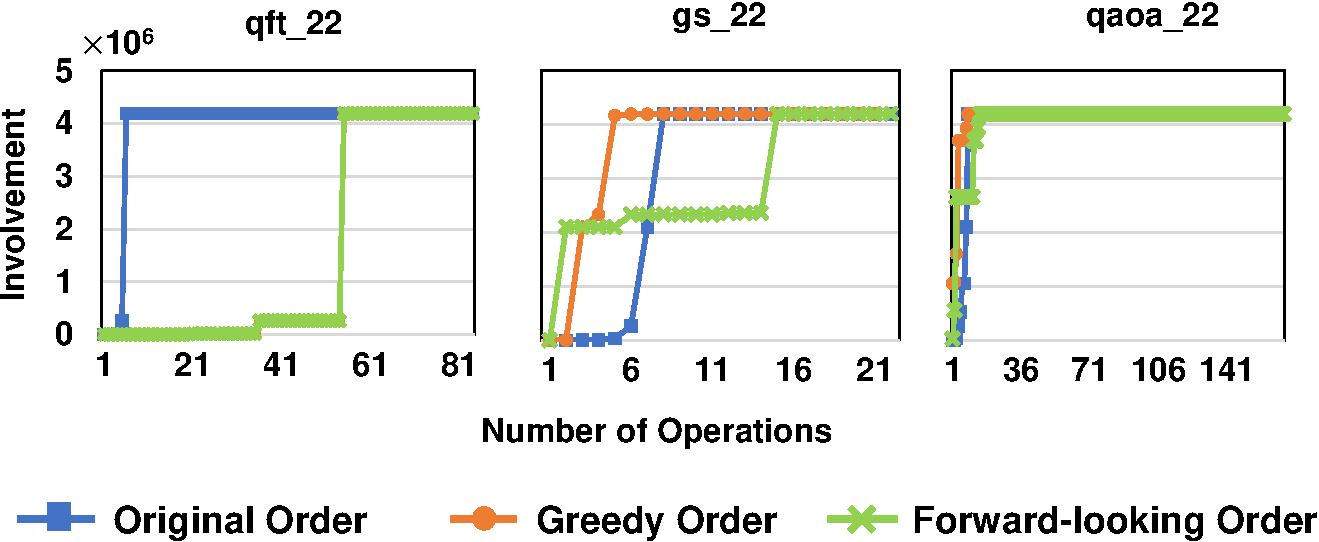
\includegraphics[width=\textwidth]{Images/appendix2/section-4/involvement.pdf}
\centering
\caption{Qubit $Involvement$ during simulation in three representative circuits.}%\xulong{I would put 10^6 on the top, next to the 50 label.}}
\label{fig-inv}
\vspace{-5pt}
\end{figure}

\noindent \textbf{Reorder effectiveness:}
To assess the performance of the reordering algorithms discussed above, we implement them to reorder the original operation sequences for all benchmark circuits that have 22 qubits and plot the $involvement$ (Algorithm \ref{alg:pruning} in Section \ref{sec:pruning}) after each gate has been applied. For the purpose of illustration, we depict the results of three representative benchmark circuits in Figure \ref{fig-inv}. 
For each order, i.e original order, greedy-reorder, and forward-looking reorder, the ``speed'' of reaching the maximum $involvement$ indicates the pruning potential. 
We observe that, forward-looking reordering results in the largest pruning potential, while greedy reordering only works for {\tt qft\_22} and even results less pruning potential than baseline for {\tt gs\_22}. Particularly. for {\tt gs\_22} and {\tt qft\_22}, forward-looking reordering effectively delays the involvement of qubits. Thus, we can expect the pruning potentials of these circuits to be enlarged by forward looking reordering. However, for {\tt qaoa\_22}, none of the reordering algorithms work due to the prevalent dependencies among the gates. Refering back to Figure \ref{fig:timeline-overlap}, when reordering (\circledwhite{V}) is employed, we can prune more chunks, which saves additional \circled{C} cycles compared to \circledwhite{IV}.  

\subsection{Non-zero State Compression}
\label{sec:compress}

\noindent {\bf Compressibility:} While pruning removes the zero state amplitudes, those non-zero amplitudes still cause data movement overheads especially for circuits that do not have large pruning potentials (e.g., {\tt qaoa} in Figure \ref{fig-inv}). Targeting reducing the data movement caused by non-zero state amplitudes, we investigate the potential compressibility and propose a GPU-supported efficient lossless data compression in Q-GPU. Specifically, we observe that many non-zero entries within a state vector, after each operation, have similar amplitude values. In other words, there is a significant ``spatial'' similarly among consecutive state amplitudes in the state vector. To demonstrate the compressibility, we use {\tt qaoa\_20} and {\tt iqp\_20} as examples and show the residuals by subtracting the consecutive state amplitudes. As one can observe from Figure~\ref{fig:residual}, for {\tt qaoa\_20}, most of the residuals are zero or very close to zero, indicating a potential for residual-based compression. However, {\tt iqp} will be less compressible due to more diverse distribution. 

\begin{figure}[h!]
    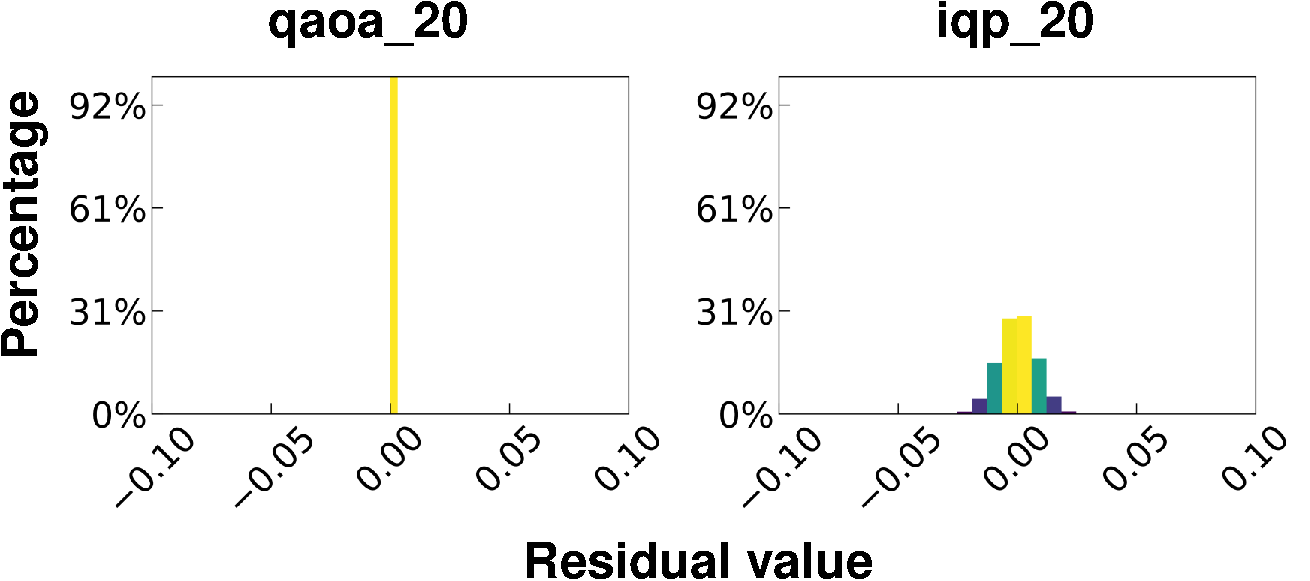
\includegraphics[width=\textwidth]{Images/appendix2/section-4/residual.pdf}
    \centering
    \caption{Residual distributions for ${\tt qaoa\_20}$ and ${\tt iqp\_20}$.}
\label{fig:residual}
\vspace{-5pt}
\end{figure}

\begin{figure}[h!]
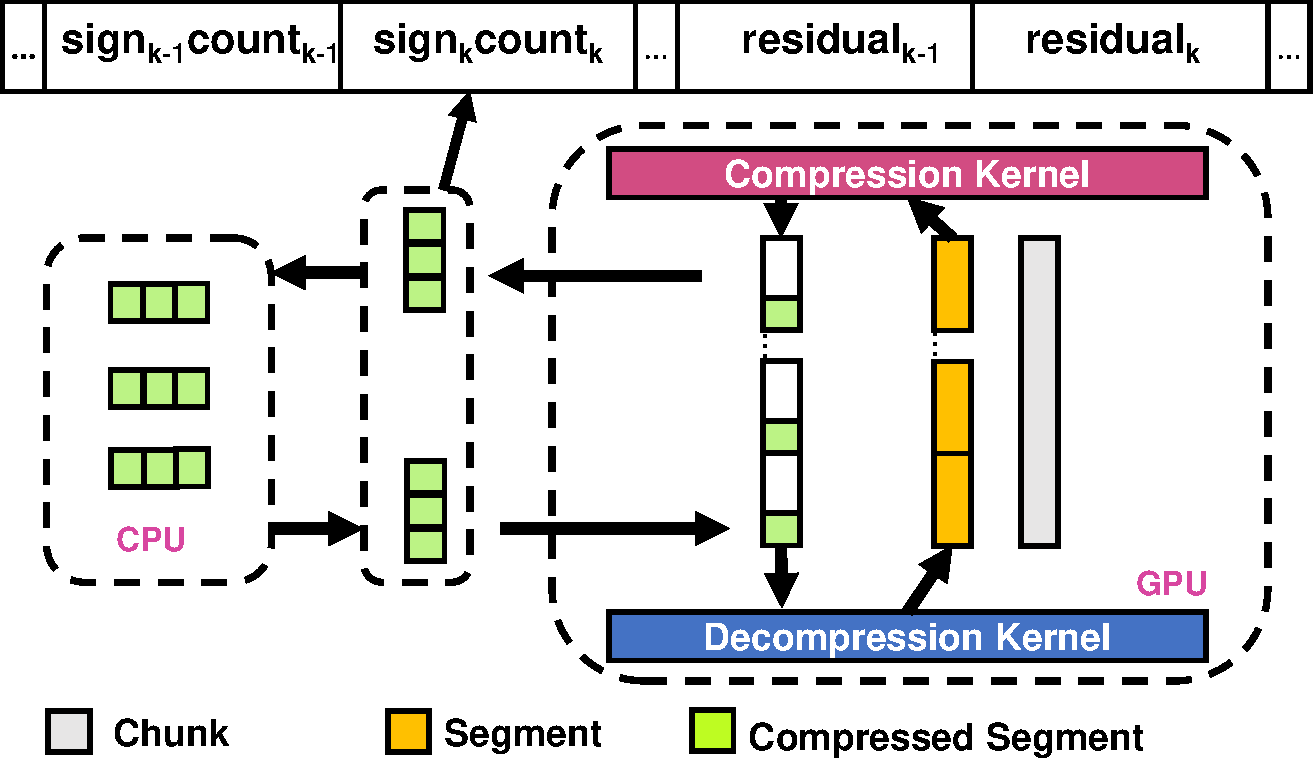
\includegraphics[width=\textwidth]{Images/appendix2/section-4/compress.pdf}
    \centering
    \caption{Overview of compression in Q-GPU.}
    \label{fig:compression-flow}
    \vspace{-5pt}
\end{figure}

\noindent \textbf{Compression Strategy:}
We use the GFC algorithm \cite{10.1145/1964179.1964189} in Q-GPU. We implement the GFC as GPU kernels to perform the compression in parallel, thereby reducing the compression and decompression overheads. Specifically, the amplitudes on the GPU are partitioned into micro-chunks with a size of 32 amplitudes. Each GPU warp iteratively compresses/decompresses in parallel. Figure~\ref{fig:compression-flow} (on the top) shows the compressed format. For the 32 values of a micro-chunk, we first store a 4-bit prefix for each of them, where one bit is used to record the sign of the residual and another three bits are a count of leading zero bytes of the residual. 
Figure \ref{fig:compression-flow} also illustrates the GPU support of compression and decompression in Q-GPU. The compression is performed on the GPU after updating the chunk before copying it to the CPU. All of the chunks are equally divided into ``segments''. We empirically choose the segment size to match the GPU parallelism such that the GPU is properly utilized during compression. The compressed segments are transferred to the CPU instead of the original state chunks. 
The CPU keeps the compressed segments and copies the compressed segments to the GPUs upon request. Once the chunks are copied to the GPU, the amplitudes are decompressed, updated, and then compressed. 
As can be seen from Figure \ref{fig:timeline-overlap}, compression (\circledwhite{VI}) saves \circled{D} cycles over \circledwhite{V} and introduces negligible overhead. Later, in section~\ref{sec:exp}, we quantify the overheads incurred by the compression and decompression procedures. 

\section{Experimental Evaluation}
\label{sec:exp}

In this section, we evaluate Q-GPU using the eight circuits in Table~\ref{tab:list-bench}. We implement Q-GPU by substantially extending IBM QISKit-Aer. The evaluation is conducted on the same CPU-GPU platform used for characterization. For all experiments, the default optimizations in QISKit-Aer are turned on in both baseline and Q-GPU evaluation. To show the effectiveness of each optimization, we test \emph{six different versions} of executions for all quantum circuit benchmarks:

\begin{itemize}

\item \emph{Baseline:}
This version is the implementation with state-of-the-art GPU support~\cite{10.5281/zenodo.2562111} in QISKit-Aer that supports GPU acceleration. As illustrated in Section \ref{sec:baseline}, state amplitudes are statically allocated on the GPU and CPU in this version. 

\item \emph{Naive:}
This version is the intuitive implementation discussed in Section  \ref{sec:naive}, which dynamically allocates state amplitudes to GPU. The performance of this version is dominated by expensive data movements.

\item \emph{Overlap:}
This version implements the first optimization -- proactive state amplitude transfer -- in Q-GPU. This version is built upon the {\it Naive} version and its details are discussed in Section \ref{sec:overlap}.

\item \emph{Pruning:}
This version adds the proposed pruning mechanism (Section \ref{sec:pruning}) to {\it Overlap}. By skipping the data movement of zero state amplitudes, the amount of data movement is reduced.

\item \emph{Reorder:}
In this version, we implement \emph{forward-looking reorder} algorithm (Section \ref{sec:reorder}) to enlarge the potential for pruning. This reordering is performed by a simple compiler pass integrated in the Q-GPU. 

\item \emph{Compression/Q-GPU:}
In this version, all optimizations are employed with compression. We also call it \emph{Q-GPU}. Compression (Section \ref{sec:compress}) is added on top of {\it Reorder}. This version achieved the best performance.


\end{itemize}

\subsection{Overall Performance}
\label{perfvali}


\begin{figure*}[t!]
	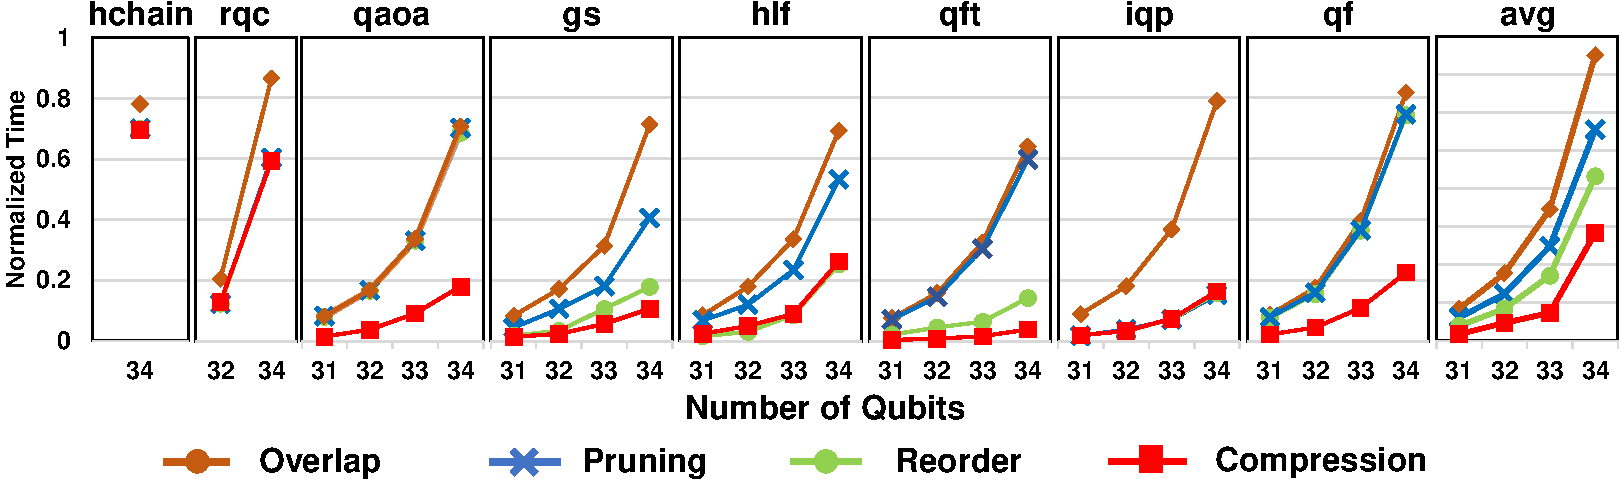
\includegraphics[width=\textwidth]{Images/appendix2/section-5/mainres.pdf}
	\centering
	\caption{Normalized simulation time for circuits with different number of qubits (the lower the better).} \label{fig:mainres}
\end{figure*} 

Figure~\ref{fig:mainres} shows the overall performance and scalability among the six versions for all eight quantum circuits. The y-axis in the figure denotes the normalized execution time to the {\it Baseline} version. From the figure, one can make the following observations. 
First, by adding the proposed optimization in Q-GPU, our approach significantly reduces the execution time of QCS  across all the circuits. 
Specifically, {\it Overlap}, {\it Pruning}, {\it Reorder}, and {\it Compression/Q-GPU} see a 24.96\%, 44.54\%, 56.78\%, and 71.66\% execution time reduction over the baseline execution for the largest number of qubits that can run on our platform. 
Second, the scalability of QCS performances is significantly improved by ``breaking'' the memory capacity in Q-GPU. 
The average achieved performance outperforms baseline by 2.53$\times$ for 34 qubits. Although we only simulate up to 34 qubits due to the CPU memory limitation (384 GB) in our system (Section \ref{sec:observation}), one can infer from the trend that our optimizations are scalable to larger sized circuits.
Third, Q-GPU has different accelerations for different circuits. Specifically, for {\tt gs}, {\tt qft}, {\tt qaoa} and {\tt iqp}, higher execution time reduction is observed, whereas for {\tt hchain} and {\tt rqc}, less speedup is observed. 
This is because, for {\tt hchain} and {\tt rqc}, reordering cannot enlarge the pruning potential because of dependent gates. Their amplitude residuals also have disperse distribution (similar to {\tt iqp} in Figure \ref{fig:residual}). Thus, either \emph{Reorder} or \emph{Compression} improves little for these two benchmarks. 
Finally, for different circuits, a certain version may not have the same acceleration effects. For example, {\it Overlap} version generates a similar execution time reduction in all circuits tested. 
However, for {\it Pruning}, {\it Reorder} and {\it Compression}, the runtime reduction is different between different circuits. For example, {\it Pruning} and {\it Reorder} improve little for {\tt qaoa} and {\tt qf} because these two circuits do not have much potential of pruning the zero amplitudes. 
That is, their qubits get involved quickly with dependent operations. However, {\tt qaoa} achieves significant benefits by compression as the great potential of compressibility. (discussed in Section~\ref{sec:compress}).


\begin{figure}[t!]
    \centering
    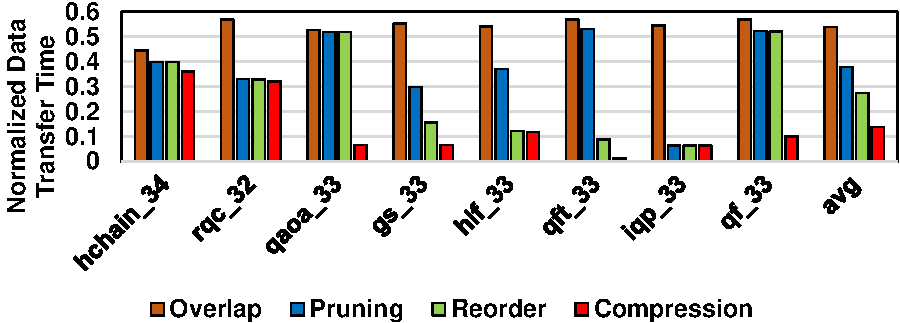
\includegraphics[width=\textwidth]{Images/appendix2/section-5/data-mov-red.pdf}
    \caption{Normalized data transfer time (lower the better).}
    \label{fig:data-mov-red}
    \vspace{-5pt}
\end{figure}


To further understand the execution reduction, Figure~\ref{fig:data-mov-red} plots, for each version, the exposed data movement time. In this figure, the y-axis represents the data movement time normalized to the {\it Naive} version. Clearly, one can observe a step-wise data movement reduction in the versions with our optimizations. 
First, {\it Overlap} uniformly reduces the data transfer time by an average of 46.14\%. Note that, the savings generated in {\it Overlap} are independent of circuit types, that is the reason behind execution time reduction in Figure~\ref{fig:mainres}. 
For {\it Pruning} and {\it Reorder}, the reduction of data movement time varies in different circuits. This is because the number of zero state amplitudes and the potential of pruning heavily rely on the circuit type. 
For example,  {\tt qaoa}, {\tt qft}, and {\tt qf} get all qubits involved at early stage of simulation. Hence, pruning is less effective for these circuits compared to others. 
Also, as discussed in Section~\ref{sec:reorder}, {\it Reorder} has little effects on {\tt hchain}, {\tt rqc}, {\tt qaoa}, and {\tt qf} due to dependent operations in these circuits. 
Therefore, {\it Reorder} delivers similar data transfer time reduction with  {\it Pruning} for these circuits. However, for those circuits with less dependent operations, {\it Reorder} significantly reduces their data movement time by enlarging the pruning potential. For circuits like  {\tt qaoa}, {\tt gs}, {\tt qft} and {\tt qf},  {\it Compression} effectively reduces the data movement by leveraging the spatial similarity discussed in Section \ref{sec:compress}. 
In a nutshell, for all circuit benchmarks tested, the reductions of data transfer time are the main reason behind the execution time reduction in Figure \ref{fig:mainres}.

We also quantify the computation time of compression and decompression in Figure \ref{fig:overhead}. Overall, the compression and decompression overhead is 3.12\% and 2.74\% of the GPU execution time. Potentially one may further optimize the compression and decompression by overlapping them on GPU, but we found the overhead is negligible compared to the significant reduction in execution time that we achieved. We also want to emphasize that the execution times reported in Figure~\ref{fig:mainres} have all the sources of overhead included.

\begin{figure}[t!]
    \centering
    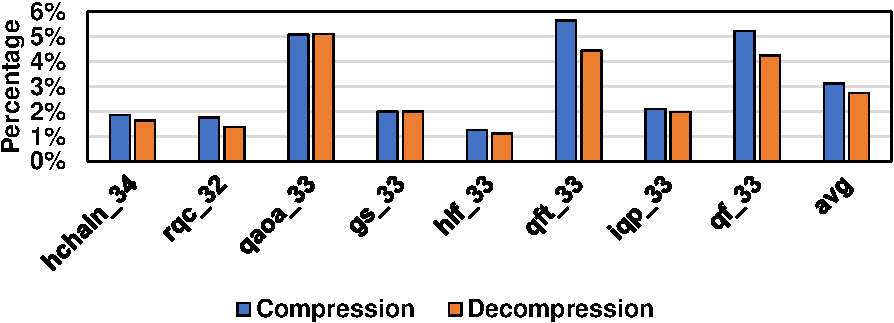
\includegraphics[width=\textwidth]{Images/appendix2/section-5/overhead.pdf}
    \caption{Compression and decompression overheads.}
    \label{fig:overhead}
    \vspace{-5pt}
\end{figure}


\subsection{Comparison with OpenMP}

\begin{figure}[h!]
	\centering
	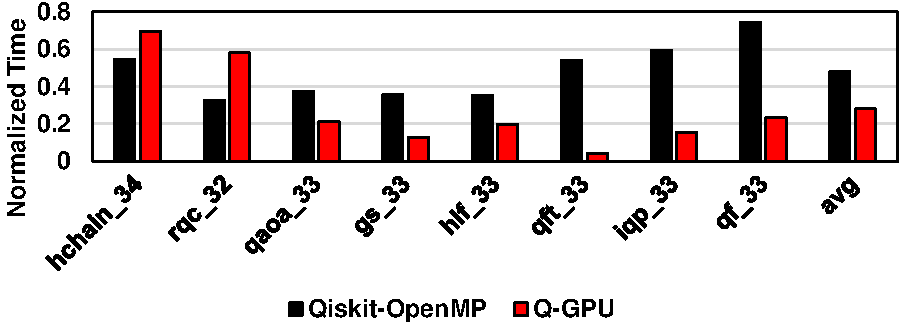
\includegraphics[width=\textwidth]{Images/appendix2/section-5/cmp-openmp.pdf}
	\caption{Comparison with OpenMP.} 
	\label{fig:cmp-openmp}
	\vspace{-5pt}
\end{figure}

Many publicly available quantum simulators and existing works employ OpenMP to parallelize the QCS on CPUs~\cite{10.48550/arXiv.1710.05867,10.1109/HPCA51647.2021.00026,10.48550/arXiv.1601.07195}. 
We compare Q-GPU with these OpenMP implementations. Specifically, we chose the OpenMP implementation in the most recent QISKit simulator and plot the results in Figure  \ref{fig:cmp-openmp}. 
We also compared our approach with other simulators in the next section, where the OpenMP is used by default in the simulators. 
On average, across eight circuits, Q-GPU outperforms the OpenMP QISKit by 1.79$\times$. Particularly, Q-GPU achieved 12.79$\times$ speedup in {\tt qft}. For {\tt gs}, {\tt iqp} and {\tt qf}, Q-GPU achieves more than 2$\times$ speedup. However, for {\tt hchain} and {\tt rqc}, Q-GPU performs worse than OpenMP. This is because the pruning potential and the compressibility are low in both circuits where Q-GPU is less effective. %\xulong{check my reason.} 


\subsection{Comparison with Other Simulators}
\label{sec:others}

\begin{figure}[h]
  \begin{subfigure}{0.5\textwidth}
    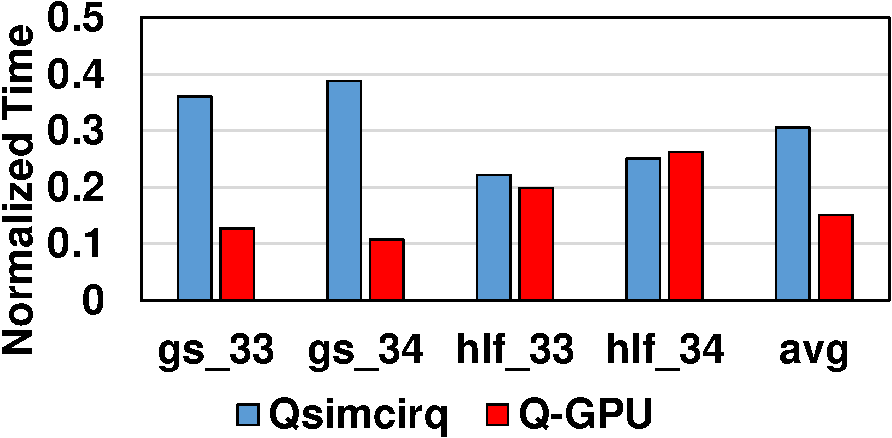
\includegraphics[width=\linewidth]{Images/appendix2/section-5/cmp-qsim.pdf}
    \caption{Comparison with Qsim-Cirq} \label{fig:qsim}
  \end{subfigure}%
\hspace{1pt}
  \begin{subfigure}{0.5\textwidth}
    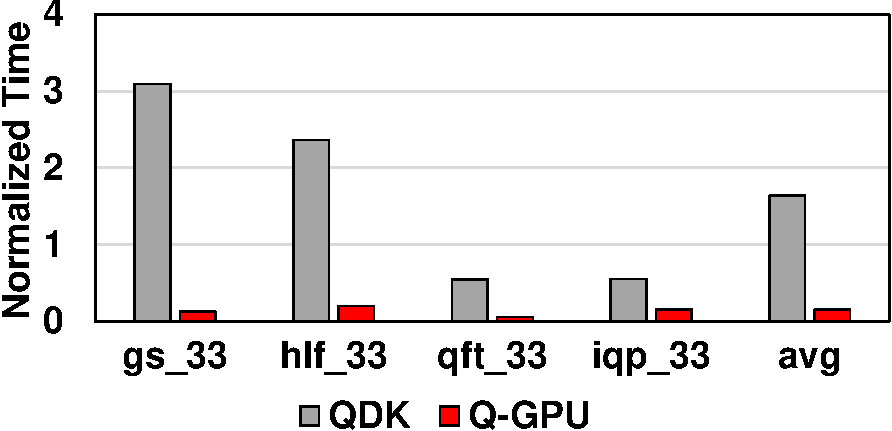
\includegraphics[width=\linewidth]{Images/appendix2/section-5/cmp-qdk.pdf}
    \caption{Comparison with QDK} \label{fig:qdk}
  \end{subfigure}%
  
\caption{Comparisons of Q-GPU to the simulator from Microsoft QDK v0.15 and Google Qsim-Cirq v0.8.0.}. 
\label{fig:others}
\vspace{-5pt}
\end{figure}

We compare Q-GPU with other simulators, including Google Qsim-Cirq v0.8.0 plus Cirq v0.9.2~\cite{10.5281/zenodo.4023103} and Microsoft QDK v0.15~\cite{msqdk}. In our experiments, we run these simulators on the same CPU (Section \ref{sec:baseline}). Note that, both Qsim-Cirq and QDK are OpenMP enabled and we observe that they used all available threads during execution on the CPU. We report the results in Figure~\ref{fig:others}. 

It is important to note that, to enable the simulation of the same circuits on Qsim-Cirq, we need to first transform our circuit benchmarks into  OpenQASM codes \cite{10.48550/arXiv.1707.03429}. Then, we need to import the OpenQASM codes to Qsim-Cirq for execution. Unfortunately, not all the transformed circuits can be simulated on Qsim-Cirq due to the lack of support for particular gates (i.e., the ``cp'' gate cannot be recognized by Qsim-Cirq). As a result, we can only run  {\tt gs} and {\tt hlf} successfully. This motivates our future research on uniform support of Quantum programming models. Figure~\ref{fig:qsim} shows the normalized speedup of the proposed Q-GPU compared to Qsim-Cirq. Q-GPU outperforms the Google Qsim-Cirq by 1.02$\times$ on average. 

To run the same quantum circuit on Microsoft QDK v0.15, we have to further convert the OpenQASM codes to ``qsharp", i.e., the quantum language used in Microsoft. The conversion only succeeded for {\tt qft}, {\tt iqp}, {\tt hlf}, and {\tt gs}. The normalized simulation time is plotted in Figure~\ref{fig:qdk}. On average, Q-GPU performs 9.82$\times$ better than Microsoft QDK. 

\section{Related Works}
\label{sec:related}
To the best of our knowledge, Q-GPU is the first work that systematically optimizes quantum circuit simulation on a GPUs. We summarize the related prior efforts below.

Prior works have focused on QCS optimizations on different platforms, from readily available devices to cloud environments~\cite{10.48550/arXiv.1601.07195,10.1145/3295500.3356155,10.48550/arXiv.1710.05867,10.1145/3126908.3126947,10.1109/HPCA51647.2021.00026,10.48550/arXiv.1910.09534,10.48550/arXiv.2005.06787,10.1109/TCAD.2018.2834427}. 
Thomas et al. \cite{10.1145/3126908.3126947} simulated 45-qubits circuit using 8,192 nodes. They optimized single node performance by using automatic code generation and optimization of compute kernels. 
Edwin et al. \cite{10.48550/arXiv.1710.05867} claimed to simulate more than 49 qubits by partitioning quantum circuits to ``subcircuits'' and delay their entanglements. 
In \cite{10.1145/3295500.3356155}, the authors proposed lossy data compression to reduce the memory requirement of simulating large-scale quantum circuits. 
Aneeqa et al. \cite{10.1109/HPCA51647.2021.00026} focused on fully exploiting single CPU performance for simulating a large number of qubits. The developed algorithm aims to reorder circuits such that more gates can be simulated in parallel.
Compared with all these efforts, Q-GPU takes advantage of GPUs while managing the data movement between CPU and GPU. 
First, we identify the source of zero state amplitudes in QCS, and propose a pruning mechanism to safely reduce unnecessary computation on these states, which saves not only computation but also data movement.
Unlike prior works using reordering to aggregate gates, \cite{10.1109/HPCA51647.2021.00026,10.1145/3498325,10.1145/3297858.3304018} 
we propose reordering algorithms to enlarge the pruning potential. Moreover, Q-GPU is the first framework that leverages the GPU to implement a lossless compression that does not affect accuracy of QCS.  Finally, it is important to emphasize that Q-GPU is complementary to existing cloud-based quantum simulation frameworks, and can be integrated within these frameworks for further QCS improvements.

There are also several works that utilize GPUs to accelerate QCS \cite{zotero-3597,10.1145/3310273.3323053,10.1007/978-3-319-68505-2_8,zotero-3528,10.1109/SC41405.2020.00017,10.1007/978-3-319-27119-4_17,10.1145/2554850.2554892}. Most of these works have limited capability in simulating large quantum circuits due to the limited memory capacity of GPUs. 
Ang et al. \cite{10.1109/SC41405.2020.00017} proposed a multi-GPU centric QCS framework that tracks the density matrix. However, their framework cannot simulate a large number of qubits since it is limited by the aggregated memory capacity of multi-GPUs. For a single-node, they can only simulate up to 14 qubits on an NVIDIA V100 GPU. 
Jun et al. \cite{10.1145/3310273.3323053} proposed a CPU-GPU co-simulation method that enables simulation using a GPU even when the required memory exceeds the GPU memory capacity. Their method is also integrated into the IBM QISKit and is used as the baseline in this paper. 
In summary, compared to prior work, Q-GPU breaks the GPU memory capacity limitation, i.e., it is able to simulate 34 qubits which require 256 GB memory on a 16 GB memory GPU, and fully takes advantage of GPU parallelization. The fundamental design innovation behind this is to dynamically and proactively transfer the state amplitudes through end-to-end optimizations to minimize the data movement overheads caused by state amplitudes transfer.  

